\documentclass{elbioimp}
\usepackage[latin1]{inputenc}
\usepackage[T1]{fontenc}
\usepackage[USenglish]{babel}
\usepackage{textcomp,graphicx}
\usepackage{lipsum}  %% For generating random text

\title{This is your template for Journal of Electrical Bioimpedance}

\author{First B. Author\affiliation{Department, University, City, Country}\and
  Second C. Coauthor\sameaffiliation\and
  Third D. Coauthor\affiliation{Xyz company}\and
  Fourth E. Coauthor\sameaffiliation[1]\and
  Last Z. Author\affiliation{E-mail any correspondence to:
    \textsf{myname@domain.com}}}

\keywords{Bioimpedance, current, voltage}

\hyphenation{bio-impe-dance}

\begin{document}
\maketitle

\begin{abstract}
  These are guidelines for preparing papers for the Journal of
  Electrical Bioimpedance. The journal accepts original research
  papers and review articles within the broad field of electrical
  bioimpedance. Use this document as a template if you are using
  \LaTeX. The paper size is A4 (21\,\texttimes\,29.7\,cm).
\end{abstract}


\section{Introduction}
This original source of this document is a template for Microsoft Word.
Please use the electronic version of this document as a
template when you produce your manuscript for submission to the
\emph{Journal of Electrical Bioimpedance}. The paper size is standard A4
(21\,\texttimes\,29.7\,cm).  

The introduction section of your paper should include the necessary
background information, including an adequate review of earlier
findings and the justification for conducting this study.


\subsection{Materials and methods}
The margins in this document are set to 2.5\,cm for the top and 1.5\,cm
for the sides and bottom. The main body of the manuscript is in two
columns separated by a 1\,cm. The line spacing is 1.1.

In the materials and methods section, please describe all necessary
details on how the study was performed. Do not include any discussions
of the work in this section. Enough information should be given so
that other researchers can reproduce your study.


\subsection{Results}
All figures should be numbered consecutively with the figure legend
indented 0.5 cm on each side.\footnote{See figure~\ref{fig:demo} for
  an example.} 

Figures may be in color or black and white and must be of such quality
that they produce clear and sharp printouts on an ordinary (color)
laser printer.

Use this section to present the results from the measurements or
studies that were described in the last section, but without going
into any discussion about the results.

\begin{figure}
  \centering
  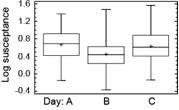
\includegraphics[width=0.8\columnwidth]{test-ill}
  \caption{Box-plot showing the median value (line), mean value (cross),
    middle 50\% (box) and smallest and largest point within
    1.5\,interquartiles from the box (whiskers) of all measurements on
    days A, B and C.\label{fig:demo}}
\end{figure}

\begin{table}
  \centering
  \renewcommand{\arraystretch}{1.2}
  \begin{tabular}{clccc}
    $D$& &$P_u$& $\sigma_N$\\
    (in)& & (lbs)& (psi)\\  \hline
     5& test 1& 285& 38.00\\
      & test 2& 287& 38.27\\
      & test 3& 230& 30.67\\  \hline
    10& test 1& 430& 28.67\\
      & test 2& 433& 28.87\\
      & test 3& 431& 28.73\\  \hline
    \end{tabular}
  \caption{A simple table\label{tab:demo}}
\end{table}

\subsection{Concluding text}
\lipsum[1-9]

\subsubsection{Additional comments}
\lipsum[10-11]


\section{Discussion}
Now you can discuss your results. Emphasize the new and important
aspects of the study and the conclusions that follow from them. Do not
repeat in detail data or other information given in the Introduction
or the Results section. After this section there may be sections
called Conclusion and Acknowledgments. The last section is
References. The \emph{Journal of Electrical Bioimpedance} uses the
Vancouver style of references with numbers in square brackets in the
text and a numbered list in the Reference section~\cite{NIH}.

\nocite{Halpern,Meltzer,Murray,Rose}
\bibliography{test-bib}
\end{document}
